One of the project's objectives was to devise a protocol for controlling the robot. Although the robot has an input for a joystick, this is insufficient for controlling the robot in a three-dimensional space. Furthermore, the platform is designed to accommodate any user requirement, necessitating the development of a protocol or language for programming the robot.

The protocol will be incorporated into the controller firmware. The commands will be transmitted in real-time by a device, currently a computer, which serves as the interface for receiving user inputs. For this reason, a command-line application has also been developed to send commands via the established port. The source code for this project, Alam\footnote{This is the name of the project. It is derived from the Spanish word "\textit{alambre}", which translates to rod or wire.}, can be found on GitHub\footnote{\url{https://www.github.com/liconaj/GraduationProject-Alam}}.

The development of the robot's kinematic model was beyond the scope of this project due to the added complexity. This remains an area for future exploration. Consequently, the control system is direct, specifying the distance or position of each actuator individually and manually. However, the intention is for this protocol to be compatible with such a model in the future.

\section{Protocol Specifications}

The G-Code is a standard language that is widely utilized in the manufacturing and computer numerical control (CNC) machining industries to control machine tools, including mills and lathes. It is composed of alphanumeric commands that specify coordinates, speeds, and machine functions. These commands facilitate precise control and automation in manufacturing processes. In addition to G-Code, M-Code commands are employed to control additional machine functions, such as tool changes and device operations.

\begingroup
\setlength{\tabcolsep}{10pt} % Default value: 6pt
\renewcommand{\arraystretch}{1.5} % Default value: 1
\begin{table}[H]
    \centering
    \caption{G-Code definitions}
    \label{tab:g-definitions}
    \begin{tabular}{p{0.1\textwidth}p{0.8\textwidth}}
    \toprule
    G-Code & Definition \\ \midrule
    \texttt{G1} & Move one or more actuators to specified positions at a given optional speed. \\
    \texttt{G4} & Pause or dwell. Halts the machine for the specified duration. \\
    \texttt{G28} & Move actuators to origin position. \\
    \texttt{G28.1} & Move actuators to target position. \\
    \texttt{G90} & Set absolute positioning mode. All subsequent movements are interpreted as absolute positions. This is the default mode. \\
    \texttt{G91} & Set relative positioning mode. All subsequent movements are interpreted as displacements from the current position. \\
    \texttt{G92} & Set origin position. \\
    \texttt{G92.1} & Set target position. This may be a position of interest. \\ \bottomrule
    \end{tabular}
\end{table}
\endgroup

The adoption of G-Code as the foundation for our robot control protocol offers efficiency and clarity, rendering it an ideal choice for rapid command transmission to microcontrollers such as the Arduino. Its hierarchical structure and diverse commands provide the flexibility needed for motion control and complex operations, aligning well with the platform's adaptability goals. The detailed definitions of the proposed G-Code and M-Code commands are presented in Tables \ref{tab:g-definitions} and \ref{tab:m-definitions}, respectively. These tables serve as a clear reference for the implementation and usage of the commands.

\begingroup
\setlength{\tabcolsep}{10pt} % Default value: 6pt
\renewcommand{\arraystretch}{1.2} % Default value: 1
\begin{table}[H]
    \centering
    \caption{M-Code definitions}
    \label{tab:m-definitions}
    \begin{tabular}{ll}
    \toprule
    M-Code & Definition \\ \midrule
    \texttt{M00} & Stop program \\
    \texttt{M85} & Maximum command wait time. \\
    \texttt{M114} & Report current position of the actuators. \\
    \texttt{M301} & Set PID parameters. \\
    \texttt{M303} & Initiate autotuning process for the PID parameters. \\
    \texttt{M355} & Report current status of robot parameters. \\
    \texttt{M500} & Save parameters to EEPROM. \\
    \texttt{M501} & Load parameters from EEPROM. \\
    \texttt{M502} & Reset parameters saved in EEPROM to defaults. \\
    \texttt{M503} & Display the saved configuration in EEPROM. \\ \bottomrule
    \end{tabular}
\end{table}
\endgroup

The application of these commands and their respective parameters is elucidated in Tables \ref{tab:g-codes-usage} and \ref{tab:m-codes-usage}. Each table includes illustrative examples that demonstrate the practical implementation of the aforementioned commands. Additionally, Table \ref{tab:code-parameters} provides a comprehensive explication of the parameters associated with each command.

\newcommand{\prompt}{\texttt{> }}

\begingroup
\setlength{\tabcolsep}{10pt}
\renewcommand{\arraystretch}{1.5}
\begin{table}[H]
    \centering
    \caption{M-Codes usage}
    \caption*{Note that only commands with parameters are explained. All others can be used by simply entering the code.}
    \label{tab:m-codes-usage}
    \begin{tabular}{p{0.1\textwidth}p{0.5\textwidth}p{0.25\textwidth}}
    \toprule
    Code & Usage & Example \\ \midrule
    \texttt{M85} & \texttt{M85 P<millis,5000>|S<secs,5>} & \prompt\texttt{M85 S3} \\
    \texttt{M301} & \texttt{M301 [P<kp,0>] [I<ki,0>] [D<kd,0>]} & \prompt\texttt{M301 P1000 I0.5} \\
    \texttt{M500} & \texttt{M500 <optn>} & \prompt\texttt{M500 T P} \\
    \texttt{M502} & \texttt{M502 <optn>} & \prompt\texttt{M502 I J K}\\
    \bottomrule
    \end{tabular}
\end{table}
\endgroup

\begingroup
\setlength{\tabcolsep}{10pt}
\renewcommand{\arraystretch}{1.5}
\begin{table}[H]
    \centering
    \caption{G-Codes usage}
    \label{tab:g-codes-usage}
    \begin{tabular}{p{0.1\textwidth}p{0.47\textwidth}p{0.28\textwidth}}
    \toprule
    Code & Usage & Example \\ \midrule
    \texttt{G1}  & \texttt{G1 <id><pos> [F<speed,255>]} & \prompt\texttt{G1 A100.0}\\
    \texttt{G4}  & \texttt{G4 P<millis>|S<secs>} & \prompt\texttt{G4 P3000}\\
    \texttt{G20} & \texttt{G20} & \prompt\texttt{G20}\\
    \texttt{G21} & \texttt{G21} & \prompt\texttt{G21} \\
    \texttt{G28} & \texttt{G28 [<id,A B C I J K>]} & \prompt\texttt{G28 A B C}\\
    \texttt{G28} & \texttt{G28.1 [<id,A B C I J K>]} & \prompt\texttt{G28.1 J K}\\
    \texttt{G90} & \texttt{G90} & \prompt\texttt{G90}\\
    \texttt{G91} & \texttt{G91} & \prompt\texttt{G91}\\
    \texttt{G92} & \texttt{G92 [<id,A B C I J K><pos,0>]}& \prompt\texttt{G92 A-100.0 I5.0}\\
    \texttt{G92.1} & \texttt{G92.1 [<id, A B C I J K><pos,0>]}& \prompt\texttt{G92.1 B250.0}\\
    \bottomrule
    \end{tabular}
\end{table}
\endgroup

\begingroup
\setlength{\tabcolsep}{10pt}
\renewcommand{\arraystretch}{1.5}
\begin{table}[H]
    \centering
    \caption{Code parameters}
    \label{tab:code-parameters}
    \begin{tabular}{p{0.2\textwidth}p{0.7\textwidth}}
    \toprule
    Parameter & Meaning \\ \midrule
    \texttt{<id>} & Actuator identification letter: \texttt{A}, \texttt{B}, \texttt{C}, \texttt{I}, \texttt{J} or \texttt{K}. \\
    \texttt{<pos>} & Position number. \\
    \texttt{<kp>} & Proportional constant. \\
    \texttt{<ki>} & Integral constant. \\
    \texttt{<kd>} & Derivative constant. \\
    \texttt{<speed>} & Maximum speed of actuator as integer number from \texttt{50} to \texttt{255}. \\
    \texttt{<millis>} & Milliseconds as integer number. \\
    \texttt{<secs>} & Seconds as integer number. \\
    \texttt{<optn>} & Parameter of the robot. \texttt{T} for PID tuning constants; \texttt{A}, \texttt{B}, \texttt{C}, \texttt{I}, \texttt{J} or \texttt{K} for position of given actuator; \texttt{P} for \textbf{all} actuator positions\\
    \texttt{<...,VALUE>} & Default value. \\
    \texttt{[...]} & Optional parameter. If omitted, default value will be used. \\
    \bottomrule
    \end{tabular}
\end{table}
\endgroup

\section{Command Line Application}

The robot's firmware was developed in Arduino/C++ using the Arduino library and the \textit{SerialCommands} library \footnote{\url{https://github.com/ppedro74/Arduino-SerialCommands}} for command definitions. Communication occurs via a serial data bus, as suggested by the name of the library. The command-line application, written in Python, employs the \textit{pyserial} library \footnote{\url{https://pypi.org/project/pyserial/}} to establish a connection with the Arduino.


\subsection{Architecture}

Figure \ref{fig:firmware-uml} depicts the dependency relationships between the firmware source components and the packages used. Furthermore, a flowchart diagram illustrating the interaction between the command-line application and the robot is included in Figure \ref{fig:system-flowchart}.

\begin{figure}[H]
    \centering
    \includesvg[width=0.95\textwidth]{firmware-uml}
    \caption{Relationships of control system components}
    \label{fig:firmware-uml}
\end{figure}


The serial port data buffer is 128 bytes, which allows for a maximum of 128 characters per command. Only a single command can be sent at a time, separated by a newline. Following the execution of a command, the robot sends a message indicating completion. The robot is programmed with a configurable maximum timeout, which is employed to handle commands that take an excessive amount of time. Ut will not interrupt or modify its current task until a new instruction is received. The robot's firmware does not support comments, and thus, these are removed by the application's parser to send only essential instructions to the robot.

\begin{figure}[H]
    \centering
    \includesvg[width=0.95\textwidth]{system-flowchart}
    \caption{System flowchart}
    \label{fig:system-flowchart}
\end{figure}


\subsection{Usage}

In order to control the robot, it is necessary to utilize the \texttt{alamctl.py} script. The code for this script can be found in Appendix \ref{apx:cli-code}. Figure \ref{fig:cli-usage} shows how to use the application via the help parameter output.


\begin{figure}[H]
    \centering
    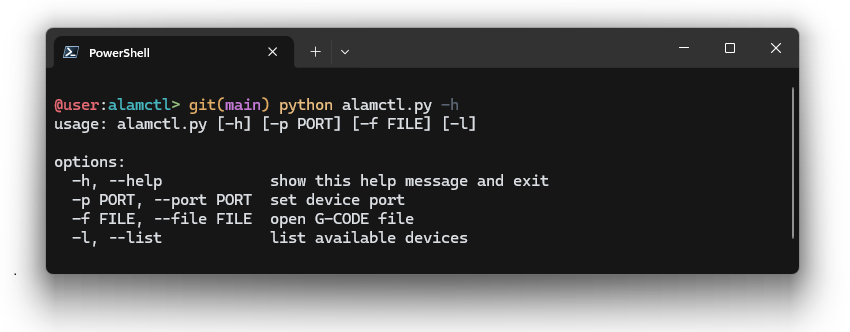
\includegraphics[width=0.85\textwidth]{cli-usage}
    \caption{Command line usage}
    \label{fig:cli-usage}
\end{figure}

It should be noted that all parameters are optional. If no parameters are passed, as explained in the flowchart in Figure \ref{fig:system-flowchart}, the application will attempt to establish a connection to one of the available ports. However, the recommended method is to initially search for available ports and then attempt to connect to the device whose description most closely aligns with that of the controller, as shown in Figure \ref{fig:cli-connection}.

\begin{figure}[H]
    \centering
    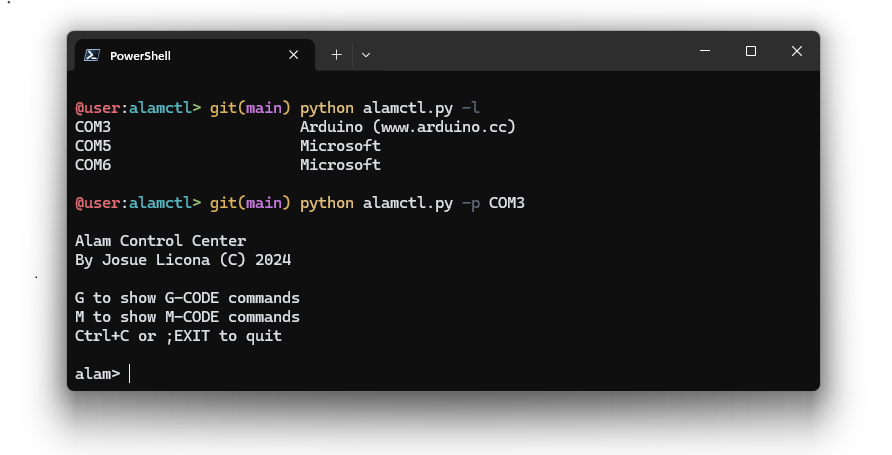
\includegraphics[width=0.85\textwidth]{cli-connection}
    \caption{Command line connection}
    \label{fig:cli-connection}
\end{figure}

Once a successful connection with the robot has been established, the application displays a welcome message and a brief instructional guide to facilitate the user's interaction with the robot (see Figure \ref{fig:cli-manual}). However, it is also possible to pass a G-Code script as a parameter for the program to send commands automatically (Figure \ref{fig:cli-file}). This is the most efficient and powerful method for users to control a robot.


\begin{figure}[H]
    \centering
    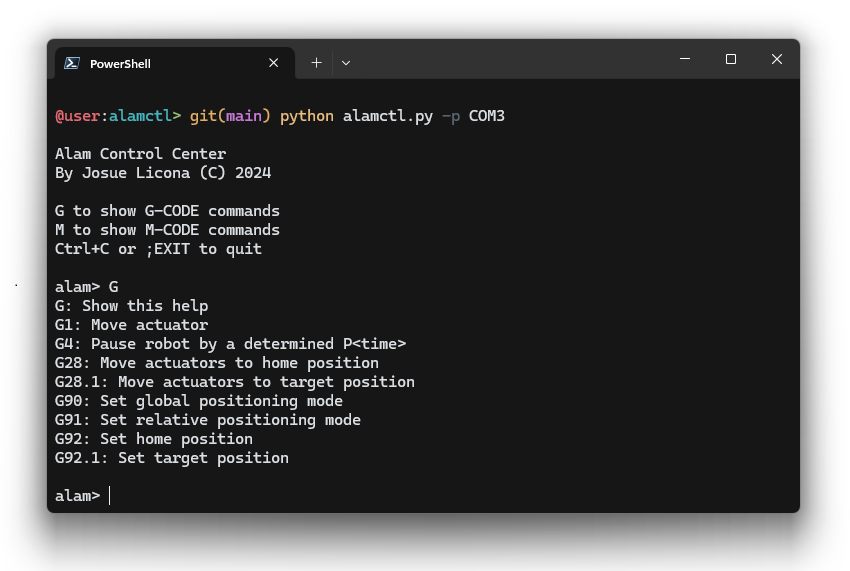
\includegraphics[width=0.85\textwidth]{cli-manual}
    \caption{Command line manual input}
    \label{fig:cli-manual}
\end{figure}

\begin{figure}[H]
    \centering
    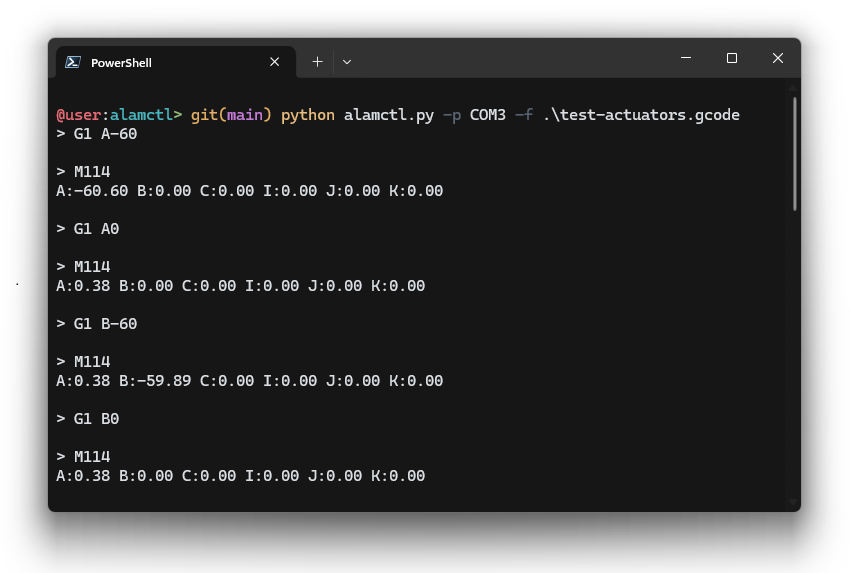
\includegraphics[width=0.85\textwidth]{cli-file}
    \caption{Command line file parsing}
    \label{fig:cli-file}
\end{figure}

\section{PID Control and Tuning}

Given that the actuators are equipped with DC motors, the controllable variable is the speed. However, the position can be determined thanks to the magnetic encoder, which counts the number of motor revolutions. Based on this, a PID control is implemented, wherein the position is utilized as the input variable, thereby enabling the controller to manipulate the speed in order to reach the desired position. To implement this control, the \textit{QuickPID}\footnote{\url{https://github.com/Dlloydev/QuickPID}} library was employed, which can be integrated with the \textit{sTune} library to determine the actuator tunings automatically. An attempt was made to use this latter library to find the tunings; however, its methods are designed for systems with an S-shaped response to a constant input, which does not apply to our system. Therefore, the outcomes yielded by this library were frequently unsatisfactory. For this reason, a more sophisticated tool, MATLAB and Simulink, was employed.

\subsection{Test Data}

\begin{figure}[h]
    \centering
    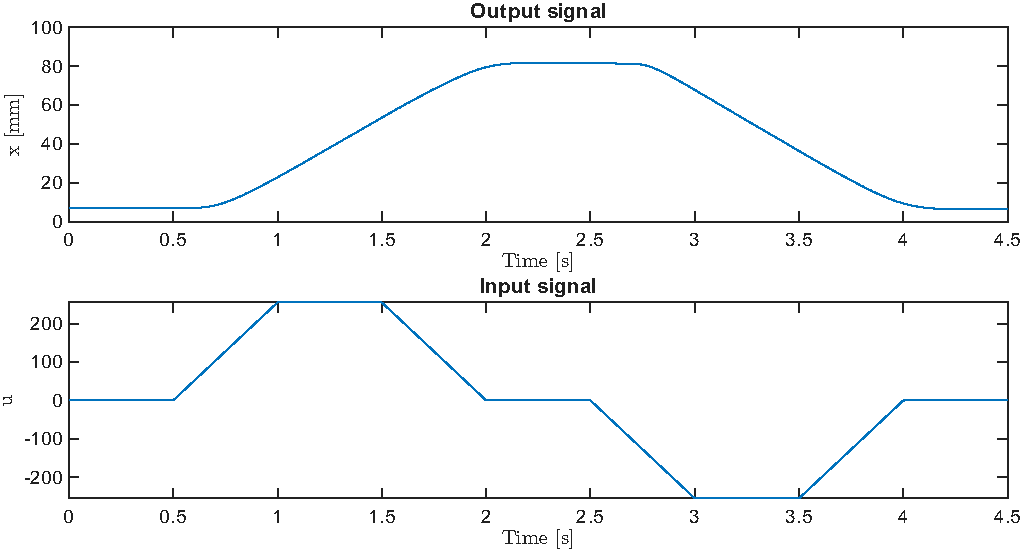
\includegraphics[page=1,width=0.85\textwidth]{input-output-signals}
    \caption{Input and output signals}
    \label{fig:io-signals}
\end{figure}

The initial step involved the implementation of a test to obtain data from the actuators, with the objective to gaining a comprehensive understanding of the system. The durations of this test is 4.5 seconds, and it can be initiated via the command \texttt{M300}. It sends a PWM signal to the actuators that varies over time. The output of the system is the linear position of the actuator at each time instant, as seen in Figure \ref{fig:io-signals}.


\subsection{System Identification}

The system's transfer function is identified based on the obtained data using MATLAB's \textit{System Identification Toolbox}. The process carried out is shown in Figure \ref{fig:tf-indent-process}. The model fit to the real data is depicted in Figure \ref{fig:tf-result}. The MATLAB code utilized is provided in Appendix \ref{apx:pid-code}.

\begin{figure}[H]
    \centering
    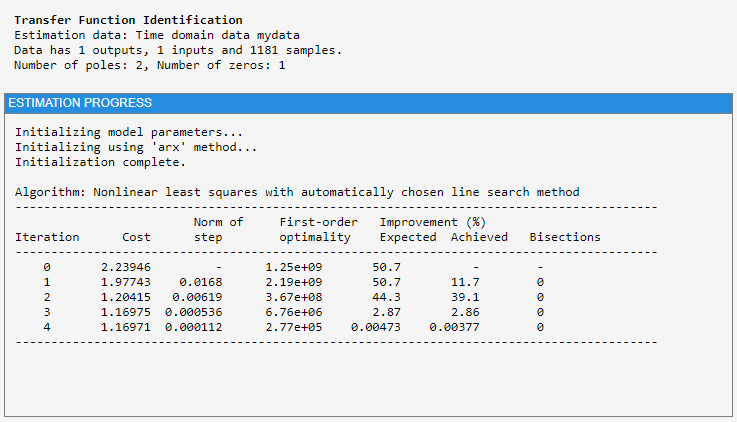
\includegraphics[width=0.65\textwidth]{tf-ident-process}
    \caption{Transfer function identification in MATLAB}
    \label{fig:tf-indent-process}
\end{figure}

\begin{figure}[H]
    \centering
    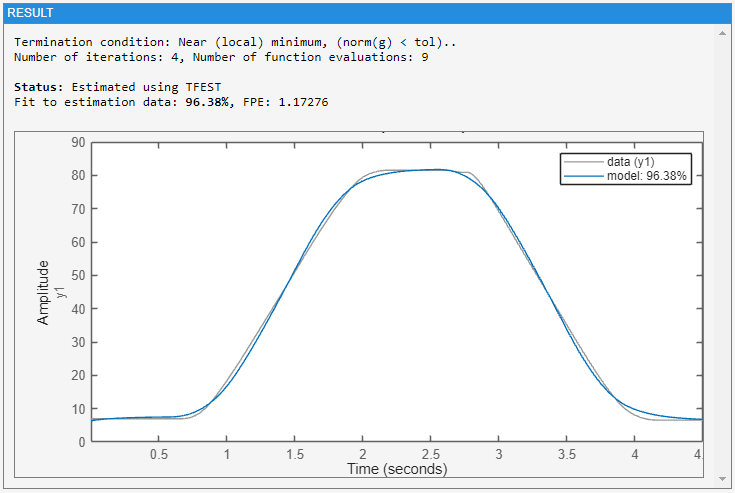
\includegraphics[width=0.65\textwidth]{tf-ident-result}
    \caption{Transfer function model in MATLAB}
    \label{fig:tf-result}
\end{figure}

The transfer equation of the linear actuator that was identified is shown in Equation \ref{eq:tf}, where the variable of the function is \( z^{-1} \).

\begin{equation}
    \label{eq:tf}
    tf=\frac{(4.808-4.596z^{-1})\times10^{-4}}{1-1.982z^{-1}+0.9824z^{-2}}
\end{equation}


\subsection{PID Tuning}

The tunings of the PID controller were determined using the MATLAB utility \textit{pidTuner}. The PI controller, which is a PID controller with $K_d = 0$, exhibited the most optimal response. In this instance, the control is discrete, and the resulting constants are presented in Table \ref{tab:pid-tunings}. These variables are utilized to implement the controller with the \textit{QuickPID} library in Arduino.

\begin{equation}
    \label{eq:pid-equation}
    C = Kp + Ki * \frac{Ts}{z-1}
\end{equation}

\begin{table}[h]
    \centering
    \caption{PID tunings}
    \label{tab:pid-tunings}
    \begin{tabular}{ll}
    \toprule
    Property & Value \\
    \midrule
    Proportional constant, $Kp$  & 21.4 \\
    Integrative constant, $Ki$ & 1.97 \\
    Sample time, $Ts$ & $0.00381$s \\
    \bottomrule
    \end{tabular}
\end{table}

\begin{figure}[H]
    \centering
    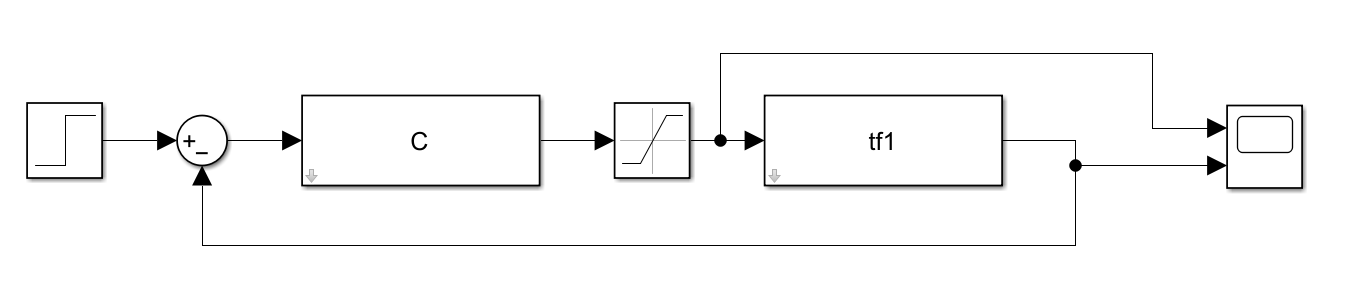
\includegraphics[width=\textwidth]{system-blocks}
    \caption{Blocks diagram of control system}
    \label{fig:system-blocks}
\end{figure}

A general block diagram of the control system is shown in Figure \ref{fig:system-blocks}, where \texttt{C} represents the transfer function of the PID controller (equation \ref{eq:pid-equation}) and \texttt{tf1} represents the transfer function of the actuator. The system's response to a 100 mm input is shown in Figure \ref{fig:system-response}. The blue curve indicates that the system responds promptly, reaching the desired value in approximately two seconds, theoretically. However, it exhibits overshoot and takes nearly four seconds to settle into a steady state. In many cases, it is not necessary for the robot to reach exact intermediate positions when it is in motion. Consequently, the firmware was programmed to permit the input of new commands once the desired position has been reached, thus compromising accuracy for speed.

\begin{figure}[H]
    \centering
    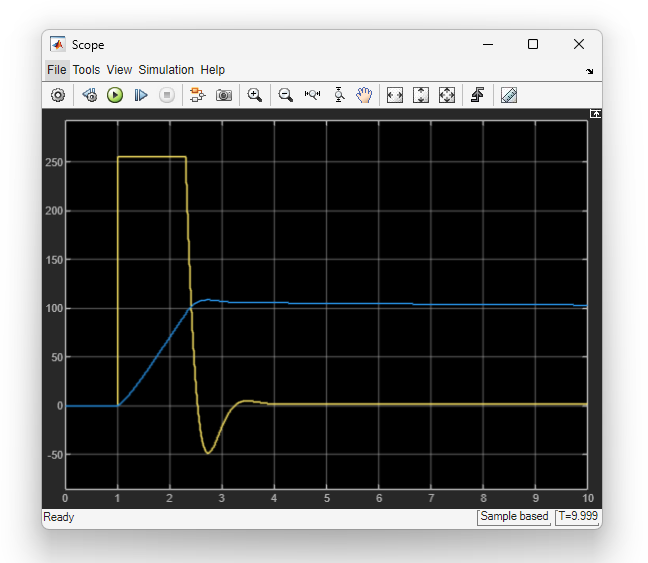
\includegraphics[width=0.6\textwidth]{system-response}
    \caption{System response of simulation in Simulink}
    \label{fig:system-response}
\end{figure}

Moreover, the control signal, depicted in yellow, exhibits saturation, underscoring the necessity to implement an anti-windup control. Fortunately, the \textit{QuickPID} library offers a function for this, rendering implementation straightforward. This feature was duly applied.
